% =====================================================================
% Supplementary Information for Paper 1 v64
% =====================================================================
\documentclass[preprint,11pt,authoryear]{elsarticle}
\usepackage{amsmath,amssymb,amsthm}
\usepackage{booktabs}
\usepackage{array}
\usepackage{tabularx}
\usepackage{graphicx}
\graphicspath{{./}{figs/}{paper1_assessment_separation_v64_src/figs/}}
\usepackage{enumitem}
\usepackage[colorlinks=true,urlcolor=blue,linkcolor=blue,citecolor=blue]{hyperref}
\emergencystretch=3em
\setlength{\tolerance}{2000}

\renewcommand{\thesection}{S\arabic{section}}
\renewcommand{\thetable}{S\arabic{table}}
\renewcommand{\thefigure}{S\arabic{figure}}
\renewcommand{\theequation}{S\arabic{equation}}
\newtheorem{theorem}{Theorem}
\renewcommand{\thetheorem}{S\arabic{theorem}}
\newtheorem{lemma}{Lemma}
\renewcommand{\thelemma}{S\arabic{lemma}}
\newtheorem{proposition}{Proposition}
\renewcommand{\theproposition}{S\arabic{proposition}}
\theoremstyle{remark}
\newtheorem{remark}{Remark}
\renewcommand{\theremark}{S\arabic{remark}}

\newcommand{\Etyp}{E_{\mathrm{typ}}}
\newcommand{\Eend}{E_{\mathrm{end}}}
\newcommand{\Ephys}{E_{\mathrm{tube,phys}}}
\newcommand{\Vtyp}{\mathcal{V}_{\mathrm{typ}}}
\newcommand{\Vweak}{\mathcal{V}_{\mathrm{weak}}}
\newcommand{\Vphys}{\mathcal{V}_{\mathrm{phys}}}
\newcommand{\Vend}{\mathcal{V}_{\mathrm{end}}}
\newcommand{\Wp}{W_+}
\newcommand{\FP}{\mathrm{FP}_{\mathrm{agg}}}
\newcommand{\Tube}{\mathrm{Tube}}
\newcommand{\Succ}{\mathrm{Succ}}
\newcommand{\End}{\mathrm{End}}
\newcommand{\conv}{\operatorname{conv}}
\newcommand{\Rp}{\mathbb{R}^n_+}
\newcommand{\Q}{\mathcal{Q}}
\newcommand{\act}[1]{\textsc{#1}}

\journal{Journal of Multi-Criteria Decision Analysis}

\begin{document}
\begin{frontmatter}
\title{Supplementary Information for:\\ Every weighting licenses a plan, no plan satisfies the floors: a quantifier-order separation between compensatory and noncompensatory transition assessment}
\author[1]{Amin Abaee}
\ead{amin_abaee@ut.ac.ir}
\affiliation[1]{organization={Independent Researcher}, city={Tehran}, country={Iran}}
\begin{abstract}
This Supplementary Information accompanies the main article. It contains the remaining proofs (S2), the substitutability-spectrum extension in full (S3), the common-shock variant in full (S4), the resource-transition benchmark in full (S5), practitioner material (S6), the verification record (S7), positioning notes per literature (S8) and the framework extensions deposited at partial status (S9). Main-text results are cited as ``main-text Theorem~2'' etc.; results stated here are numbered S1, S2, \dots. Every number is an exact rational (or a certified rational bracket of a transcendental quantity) re-derived by the deposited verification code. Nothing in this document is an empirical claim, and no main-text proof depends on S3--S9.
\end{abstract}
\end{frontmatter}

\section{Abbreviations and the result map}

\begin{table}[!htbp]
\centering\small
\caption{Abbreviations.}
\begin{tabular}{@{}ll@{}}
\toprule
CES & constant elasticity of substitution \\
DFO & Fisheries and Oceans Canada \\
LPI & Living Planet Index \\
LRP & limit reference point \\
MCDA & multi-criteria decision analysis \\
MSY & maximum sustainable yield \\
NCAM & Northern Cod Assessment Model \\
SI & Supplementary Information \\
\bottomrule
\end{tabular}
\end{table}

\begin{table}[!htbp]
\centering\small
\caption{Map between the main-text result numbers (v64) and the numbering of the previous editions (v62 and v63, which share one numbering), for readers of the deposited verification code and the Lean module, whose comments use the v62 numbers.}
\begin{tabularx}{\textwidth}{@{}>{\raggedright\arraybackslash}p{0.42\textwidth}>{\raggedright\arraybackslash}p{0.24\textwidth}X@{}}
\toprule
Main text (v64) & Previous editions (v62/v63) & Verifier / Lean reference \\
\midrule
Lemma 1 (quantifier inclusion) & Remark 1 & -- \\
Lemma 2 (full cone lossless) & Remark 2 & Lean: full-cone identity \\
Proposition 1 (hierarchy, localisation) & Proposition 3 & grid check 10, 19; Lean \\
Proposition 2 (weight-family monotonicity) & Proposition 4 & -- \\
Theorem 1 (finite-menu geometry) & Theorem 6 & -- \\
Theorem 2 (witnessed separation) & Theorem 5 & grid checks 5--9, 11--22; Lean \\
Proposition 3 (persistence, erasure) & Remark 7, Theorem 8 & grid checks 23--25 \\
Theorem 3 (blend collapse) & Theorem 9 & Lean \\
Proposition 4 (time-sharing) & Proposition 10 & Lean \\
Proposition 5 (rescue threshold) & Proposition 11 & grid check 22 \\
Theorem 4 (substitutability ladder) & Lemma A, Lemma B, Theorems S1, S2 & $\sigma$-verifier (57 checks); Lean \\
Proposition 6 (common-shock verdict) & Theorems M1, M2, M3 & common-shock verifier (77 checks) \\
S3.2 Theorem S3 (off-diagonal criterion) & Theorem G & closure verifier (50 checks) \\
S4 Theorems S6--S7 & Theorems M4, CT & common-shock verifier \\
\bottomrule
\end{tabularx}
\end{table}

\section{Remaining proofs}\label{si:proofs}

\subsection{Persistence under hold-prefix extension (main-text Proposition 3(i))}

\begin{proof}
(Hierarchy.) Backward induction on stages. Base: at the final stage the terminal sets satisfy $G\subseteq G^w\subseteq G^{\mathrm{phys}}$ by main-text Lemma~2 and the definition of the terminal sets. Step: the accepted set of a stage is the set of states from which some action keeps the tube in the safe set and the successor in the next-stage accepted set; applying main-text Proposition~1(i) to the stage's action sets and the induction hypothesis to the next-stage accepted sets preserves the three-way inclusion at the stage level.
(Persistence of strictness.) With \act{hold} the unique prefix action, a prefix state is accepted exactly when it lies in the prefix safe set and in the next-stage accepted set; the stage-0 regions are therefore the witness regions of main-text Theorem~2 pulled back through the (identity) holds, and the strictness witnesses ($I\neq\varnothing$ and the point $(\tfrac12,\tfrac1{10},\tfrac1{10})$) persist.
(Conditionality.) Each of the three mechanisms listed in the main text -- a common typed-safe continuation for every aggregate-feasible state, coincident weak and typed terminal sets on the reachable subset, or actions coupled across stages -- is sufficient to erase the gap in a multi-stage setting, so no unconditional generalisation is asserted.
\end{proof}

\subsection{The erasure datum (main-text Proposition 3(ii))}\label{si:erasure}

\emph{Datum.} Two capital forms, floors at zero, the bridge stock absent ($x\equiv0$); states are pairs $s=(s_1,s_2)$. Stage 2 (final interval): safe set $S_0^{(2)}=\mathbb R^2$ (no path constraint), terminal sets $G^{(2)}=G^{w,(2)}=G=\{s\ge0\}$ -- coincident for every weight -- and a single action \act{repair} with tube $\{s\}$ and successor $(1,1)\in G$. Stage 1: safe set $S_0=\{s\ge0\}$; two actions with constant tubes, safe at every state of $S_0$: A1 with successor $(s_1-1,s_2+1)$ and A2 with successor $(s_1+1,s_2-1)$; the stage-1 terminal architecture is the stage-2 accepted sets. Initial state $z^*=(\tfrac25,\tfrac25)$.

\emph{In the two-stage datum the gap is erased.} \act{repair} is typed-admissible -- hence $w$-admissible for every weight -- from every state, so $\mathcal V^{(2)}_{\mathrm{typ}}=\mathcal V^{(2)}_w=\mathbb R^2$ for every $w$. Backward induction then admits both A1 and A2 at $z^*$ (safe tubes; successors in $\mathbb R^2$), so $z^*$ is typed-accepted at stage 0, and weak acceptance follows.

\emph{In the single-interval truncation the gap is present.} With the final interval collapsed to its terminal sets $G=\{s\ge0\}$ and $G^w=\{w\cdot s\ge0\}$, both successors leave $G$ ($s_1-1=-\tfrac35<0$ and $s_2-1=-\tfrac35<0$), so $z^*$ is typed-rejected. For the weak doctrine, with $r=w_2/w_1$ on the interior of the cone: A1 is $w$-admissible exactly when $(s_1-1)+r(s_2+1)\ge0$, i.e.\ $r\ge\tfrac{1-s_1}{s_2+1}=\tfrac37$; A2 exactly when $(s_1+1)+r(s_2-1)\ge0$, i.e.\ $r\le\tfrac{s_1+1}{1-s_2}=\tfrac73$; the two intervals cover $[0,\infty]$ because $\tfrac37<\tfrac73$, and the boundary weights are covered directly. Hence $z^*\in\Vweak$ in the truncation and the gap contains $z^*$. \qed

\subsection{The substitutability ladder (main-text Theorem 4)}\label{si:ladderproofs}

Notation as in main-text Section~4.5: $\lambda_i=1+s_i$, normalised weights $w$, $M_\theta(\lambda;w)=(\sum_iw_i\lambda_i^\theta)^{1/\theta}$, $\sigma=1/(1-\theta)$.

\begin{lemma}[the handshake]\label{lem:handshake}
With weights normalised, $\sum_iw_i\lambda_i\ge1\iff w\cdot s\ge0$; the $\theta=1$ member therefore reproduces the compensatory operator of the main text exactly -- the same acceptance set at every state and weight, and at the witness point the same per-weight plan assignment ($\rho_1=2/3$, $\rho_2=3/2$).
\end{lemma}
\begin{proof}
$\sum_iw_i\lambda_i=\sum_iw_i+\sum_iw_is_i=1+w\cdot s$.
\end{proof}

\begin{lemma}[collapse convention]\label{lem:collapse}
For every $\theta<1$ member, any tube value $\lambda_i\le0$ rejects the plan: a coordinate at or below the collapse level cannot be compensated by surpluses elsewhere.
\end{lemma}
\noindent The geometric mean is $0$ there, CES with $\theta<0$ is undefined there, and for $\theta\in(0,1)$ the convention is the family's defining property. The $\theta=1$ member alone compensates across collapse: at the witness point \act{fast}'s trough has $\lambda=(1/5,11/5)$, and the linear member certifies it at equal weight ($6/5\ge1$) while every $\theta<1$ member with a collapsed coordinate elsewhere rejects (e.g.\ at $(1/2,1,1)$, where the trough has $\lambda_1=0$).

\paragraph{The master equation} On the diagonal $z=(x<1,s,s)$ with $s\in(1,2)$, \act{fast}'s worst-case trough is $\lambda=(s-1,s+1)$ and \act{slow}'s is $(s+1,s-1)$; \act{staged} is inadmissible ($x<1$). Write $p=w_1$ for the weight share, $A=(s-1)^\theta$, $B=(s+1)^\theta$. For $\theta>0$, \act{fast} is accepted at $p$ iff $pA+(1-p)B\ge1$ and \act{slow} iff $pB+(1-p)A\ge1$; both are affine in $p$ and sum to $A+B$. \act{fast}'s acceptance set is a downward interval $[0,p_F]$ (its condition is decreasing in $p$ since $A<B$) and \act{slow}'s an upward interval $[p_S,1]$, with $p_S=1-p_F$ by symmetry; the cover $[0,p_F]\cup[p_S,1]=[0,1]$ holds iff $p_F\ge\tfrac12$, i.e.\ iff the condition holds at $p=\tfrac12$: $(A+B)/2\ge1$. For $\theta<0$ the inequality $M_\theta\ge1$ reads $\sum w_i\lambda_i^\theta\le1$ and the same argument gives $(A+B)/2\le1$. For $\theta=0$ the condition is $(s-1)^p(s+1)^{1-p}\ge1$ with the cover at $p=\tfrac12$: $s^2-1\ge1$. This is the averaging argument: the two plan conditions sum to a weight-independent quantity, so the equal weight is always the binding one.

\begin{proof}[Proof of main-text Theorem 4]
(i) \emph{Nesting.} For fixed positive $\lambda$ and weights, $M_\theta$ is nondecreasing in $\theta$ (the power-mean inequality); the collapse convention preserves this, since acceptance at any $\theta'<1$ forces $\lambda>0$ on the serving plan's tube, where the family is defined. Per plan and weight, hence per weight, hence for the protocol: acceptance at $\theta'$ implies acceptance at every $\theta>\theta'$, so the accepted rungs form a prefix and $\sigma^*(z)$ is well defined. \emph{Finiteness} on gap states with both coordinates in $(1,2)$: at the equal weight, \act{fast}'s condition contains the term $(s_1-1)^\theta$ and \act{slow}'s the term $(s_2-1)^\theta$, both of which tend to $\infty$ as $\theta\to-\infty$ because $s_i-1<1$; so for some finite $\theta$ neither plan serves the equal weight and the state is rejected (on the diagonal this is $(s-1)^\theta\to\infty$). \emph{Positivity}: $s_1+s_2\ge2$ accepts at $\theta=1$. \emph{Only-linear states}: if $\min(s_1,s_2)\le1$, say $s_1\le1$, then \act{fast}'s trough has $\lambda_1=s_1-1\le0$ and is rejected at every $\theta<1$ by Lemma~\ref{lem:collapse}; \act{slow} alone must then cover every weight, including the weight concentrated on coordinate $2$, where its condition is $s_2-1\ge1$, i.e.\ $s_2\ge2$, excluded on a gap state. So only the linear member certifies and $\sigma^*=\infty$.
(ii) Immediate from (i): every gap state is linear-accepted, the accepted rungs form a prefix, and finiteness (or only-linearity) supplies a positive elasticity at which the state is rejected.
(iii) Evaluate the master comparison at $s=2$: for $\theta\in(0,1)$ the accepting side is $\ge2$ and $(s-1)^\theta+(s+1)^\theta=1+3^\theta>2$ strictly; for $\theta<0$ the accepting side is $\le2$ and $1+3^\theta<2$ strictly; for $\theta=0$, $4>2$. All strictly accepting at $s=2$, so by continuity some $\varepsilon>0$ has every $s\in(2-\varepsilon,2)$ accepted at that rung, and these are gap states (typed acceptance needs $s\ge2$); the acceptance condition is monotone in $s$ on $(1,2)$ (both $A$ and $B$ move the accepting way), so the accepted set is exactly $[s^*(\theta),2)$ with $s^*(\theta)<2$. The closed forms of main-text Table~4 follow by direct evaluation ($\theta=1/2$: $\sqrt{s-1}+\sqrt{s+1}\ge2$, equality at $s=5/4$; $\theta=0$: $s^2\ge2$; $\theta=-1$: $(s^2-1)/s\ge1$; $\theta=-2$: $(s+1)^2+(s-1)^2\le2(s^2-1)^2\iff s^2\ge3$; $\theta=-m$: $(s-1)^{-m}+(s+1)^{-m}\le2$), and strict monotonicity of $s^*$ in depth is the nesting of (i) applied to the critical floors. The Leontief member's acceptance is weight-independent ($\min_i\lambda_i\ge1$ does not involve $w$), so its protocol collapses into the common-plan criterion -- the typed operator; hence $\inf_z\sigma^*(z)=0$ and only $\sigma=0$ is uniformly safe.
\end{proof}

\subsection{The common-shock verdict (main-text Proposition 6)}\label{si:csproofs}

The variant is defined in main-text Section~4.6 and S4 below. Write $A(p)=ps_1+(1-p)s_2$ for the aggregate margin at weight share $p$.

\begin{proof}[Proof sketch (machine-anchored)]
(i) \act{fast}'s common-class requirement is $A(p)\ge\max(2p,\ p+\tfrac12)$ (its own tent $3/2$ in $s_1$ plus the $s_1$-event, and the $s_2$-event weighted by $1-p$); \act{slow}'s is the mirror; \act{staged}'s ($x\ge1$) is $A(p)\ge\max(p,1-p)/2-1/8$, the event exposure of a growing floor (kinked in $p$; its admissibility decomposes exactly into the two affine conditions of the kink's branches). The pointwise minimum of the two principal requirements is a tent with its only kink at $p=\tfrac12$, so an affine $A$ covers it exactly at the three abscissae $p\in\{0,\tfrac12,1\}$; the closed forms follow: typed acceptance needs $s_1\ge2$ with $s_2\ge\tfrac12$ (or the mirror) or the staged branch $x\ge1$, $\min(s)\ge\tfrac38$; weak acceptance with $x<1$ needs $s_1\ge\tfrac12$, $s_2\ge\tfrac12$ (the endpoints $p=0,1$) and $s_1+s_2\ge2$ (the kink). The licensing endpoint of \act{fast} on the surviving region equals its action-indexed endpoint $1/(1+\rho_1)$, since the binding branch there is the own-tent branch. The verifier checks the closed forms against independent grid computations ($5{,}000$-state grids) plus a curated witness list, both directions.
(ii) The augmented menu adds $\act{staged}_\kappa$, admissible at $x+\kappa\ge1$ with the same floor requirement $s_i\ge\tfrac38$; $\kappa$ cannot move the floors, so on $\{\min(s)<\tfrac38\}\setminus\Vtyp^{\mathrm{cs}}$ no finite $\kappa$ certifies. On the complement the requirement is the action-indexed one, $\kappa=(1-x)_+$. The $3/8$ boundary is structural: the event exposure of a growing floor is $\max(0,\delta-1/8)=3/8$ at $\delta=1/2$.
(iii) The blend's $s_1$-trough is $s_1-\delta-\delta_{\mathrm{blend}}\cdot\tfrac32$ and its $s_2$-trough $s_2-\delta-(1-\delta_{\mathrm{blend}})\cdot\tfrac32$ (each coordinate takes its event plus the corresponding fraction of the principal tent); the window is the nonnegativity interval of the two intersected with $[0,1]$, nonempty iff $s_1\ge\delta$, $s_2\ge\delta$ and $s_1+s_2\ge\tfrac32+2\delta$.
\end{proof}

\section{The substitutability spectrum in full}\label{si:spectrum}

This section carries the full record of the CES extension summarised in main-text Section~4.5 and Theorem~4. All results are stated on the witness datum and inherit its scope delimitations; $\sigma$ denotes the elasticity of substitution throughout (the Schaefer surplus of the benchmark is written $\varsigma$).

\subsection{The critical-elasticity landscape on the diagonal}

For each gap state the accepted rungs form a prefix of the ladder (main-text Theorem~4(i)), so the $\sigma$-aggregator falsely certifies $z$ exactly when $\sigma\ge\sigma^*(z)$. Table~\ref{tab:sigmastar} lists exact brackets on the diagonal $x=1/2$; Figure~4(b) of the main text overlays them on the master-equation root.

\begin{table}[!htbp]
\centering\small
\caption{The critical elasticity $\sigma^*(z)$ on diagonal gap states $z=(1/2,s_1,s_2)$ (exact brackets; strict at both ends unless noted).}
\label{tab:sigmastar}
\begin{tabular}{@{}llp{6.4cm}@{}}
\toprule
state $z=(x,s_1,s_2)$ & $\sigma^*(z)$ & note \\
\midrule
$(1/2,\,1,\,1)$ & $\infty$ exactly & only the linear member certifies \\
$(1/2,\,3/2,\,1/2)$ & $\infty$ exactly & min coordinate $\le1$: only-linear \\
$(1/2,\,6/5,\,6/5)$ & $\in(2,3)$, strict & the witness point \\
$(1/2,\,5/4,\,5/4)$ & $=2$ exactly & the $\theta=1/2$ rung's equality state \\
$(1/2,\,13/10,\,13/10)$ & $\in(1,2)$ & \\
$(1/2,\,3/2,\,3/2)$ & $\in(1/2,1)$, strict & the LPI-form witness \\
$(1/2,\,13/8,\,13/8)$ & $\in(1/3,1/2)$ & the harmonic member's false-certification witness \\
$(1/2,\,9/5,\,9/5)$ & $\in(1/5,1/4)$ & \\
$(1/2,\,39/20,\,39/20)$ & $\in(1/17,1/13)$ & near the typed boundary: $\sigma^*\to0$ \\
\bottomrule
\end{tabular}
\end{table}

Gap states with $\min(s_1,s_2)\le1$ are only-linear ($\sigma^*=\infty$); states with both coordinates $>1$ have finite $\sigma^*$, given on the diagonal by the master-equation root, with $\sigma^*(s)\to0$ as $s\to2^-$ and $\sigma^*(s)\to\infty$ as $s\to1^+$. Concretely, $\sigma=3$ certifies $s=6/5$, $\sigma=2$ certifies $s=13/10$, $\sigma=1$ certifies $s=3/2$, $\sigma=1/2$ certifies $s=13/8$ and $\sigma=1/4$ certifies $s=9/5$ (the per-rung false-certification witnesses of main-text Theorem~4(iii)); the harmonic member's Fibonacci pair is $8/5$ rejects, $13/8$ accepts.

\subsection{The exact off-diagonal criterion}

Off the diagonal the geometric member's cover comparison is log-transcendental. It is nevertheless \emph{decided}, by certified rational enclosures: every logarithm is bracketed between two rationals carrying a checkable certificate (the all-positive-term $\operatorname{artanh}$ series for $\ln$, its tail dominated geometrically), every fractional power by integer $k$-th-root brackets, and every cover comparison is multilinear in the enclosed quantities, so its extrema over the enclosure box are attained at vertices -- a finite rational computation. Under the fail-loud discipline (any cell the schedule cannot decide aborts the run), zero cells remain undecided.

\begin{theorem}[the exact off-diagonal criterion]\label{thm:offdiag}
On the viable gap quadrant -- $x<1$, both coordinates in $(1,2)$ -- the geometric member's cover comparison reduces, by cross-multiplication of the two plans' weight thresholds, to
\[
\mathrm{cover}\iff A\cdot D\le B\cdot C,
\]
with $A=\ln(s_1-1)$, $B=\ln(s_2+1)$, $C=\ln(s_1+1)$, $D=\ln(s_2-1)$;
equivalently $r(s_1)\,r(s_2)\le1$ with $r(s)=\ln\!\big(1/(s-1)\big)/\ln(s+1)$, so the acceptance region is $\{s_2\ge\rho(s_1)\}$, where $\rho=r^{-1}\circ(1/r)$ is a strictly decreasing involution with the unique fixed point $\rho(\sqrt2)=\sqrt2$ (exactly: $r(s)\le1\iff s^2\ge2$) and limits $\rho(s)\to2^-$ as $s\to1^+$, $\rho(s)\to1^+$ as $s\to2^-$. The pivot has two sides: $\min(s_1,s_2)\ge\sqrt2$ is sufficient for the cover, and the cover forces $\max(s_1,s_2)\ge\sqrt2$; the residual wedge $\{\min<\sqrt2<\max\}$ is split by the transcendental curve $\rho$. A coordinate $s_i\ge2$ accepts outright (its own plan's worst tube keeps both coordinates at or above $1$). For the interior rungs $\theta\in(0,1)$ the same cross-multiplication, applied to $A=(s_1-1)^\theta$, $B=(s_2+1)^\theta$, $C=(s_1+1)^\theta$, $D=(s_2-1)^\theta$, gives the multilinear form $F=C(B-1)+A(1-D)-(B-D)\ge0$, which reduces on the diagonal to the master equation.
\end{theorem}

\begin{proof}[Proof sketch (machine-anchored)]
\act{fast}'s per-weight acceptance set is the downward interval $[0,U]$, \act{slow}'s the upward interval $[L,1]$, with $U=B/(B-A)$ and $L=-D/(C-D)$ at the geometric member (both denominators positive on the quadrant); the cover is $L\le U$, and the cross-multiplication is the criterion. The function $r$ is strictly decreasing (numerator decreasing, denominator increasing), so $\rho$ is well defined and strictly decreasing, and the criterion's symmetry makes it its own inverse. The enclosure lemmas certify the four quantities -- and the four powers -- between rationals; the comparison forms are multilinear, so the vertex ranges decide; every rejection additionally carries an exhibited rational witness weight served by neither plan, cross-validated in both directions against the independent per-weight algebra.
\end{proof}

\paragraph{The residual cells decided} Two wedge witnesses certify that the residual was genuine: $(5/4,3/2)$ and its mirror \textbf{reject}, with certified margins $\approx0.218$ and exhibited rational witness weights served by neither plan, while $(5/4,7/4)$ and its mirror \textbf{accept}, with margins $\approx0.422$ -- no per-coordinate rational condition separates them; the curve $\rho$ does. Together with the six $(5/4,\ge2)$-family cells, accepted by the $s_i\ge2$ boundary argument, all ten undecided cells of the 64-state grid are decided with certified strict verdicts. With the geometric member decidable off the diagonal and the interior rungs $\theta=1/2$ and $2/3$ given the same treatment, all 13 rungs are decided at all 64 grid states: the accepted rungs form a prefix at every state, the acceptance regions are up-closed in each coordinate ($\sigma^*(z)$ is nonincreasing in $s_1$ and in $s_2$), and the diagonal closed forms are reproduced. The nine finite-$\sigma^*$ states of the core $\{5/4,3/2,7/4\}^2$ form clean off-diagonal bands mirroring the diagonal ladder: $(5/4,3/2)$ and its mirror in $(1,2)$; $(5/4,7/4)$ and its mirror in $(1/2,1)$; $(3/2,7/4)$ and its mirror in $(1/3,1/2)$; $(7/4,7/4)$ in $(1/4,1/3)$; off-grid, $(6/5,7/5)$ and $(13/10,3/2)$ lie in $(1,2)$. The remaining thirteen gap states of the grid are only-linear.

\subsection{The fixed-sum tolerance structure}

Slice the gap quadrant by total margin $s_1+s_2$ (the anti-diagonals). A slice's balanced point accepts at the geometric member exactly when $s_1=s_2\ge\sqrt2$, and the $s=1$ edge accepts exactly from total $3$ up; below total $3$ the near-edge rejects. On the scanned grids the slices assemble into four regimes: \textbf{R1} (totals $\le141/50$, the witness total $12/5$ among them): every scanned point rejects; \textbf{R2} ($141/50<$ total $<2\sqrt2$; exemplar $707/250$): the balanced point rejects, moderate asymmetry accepts, the edges reject; \textbf{R3} ($2\sqrt2\le$ total $<3$; exemplar $71/25$): the balanced point accepts, strong asymmetry rejects; \textbf{R4} (totals $\ge3$): the whole slice accepts. The ecological content of the interior window: \emph{moderate concentration of a deficit is more certifiable than balance} below $2\sqrt2$.

\paragraph{The anchor decision: distribution versus total} The benchmark's asymmetric-allocation licensing choice fixes the total margin at $s_1+s_2=707/250$ (total biomass $1707/250$ kt at the floor $B_{\mathrm{lim}}=2$ kt per stock) and asks how the verdict depends on the allocation of the deficit across the stocks. Both allocations are gap states, and the LPI-structured composite rejects the balanced allocation $(707/500,707/500)$ by the diagonal closed form -- $(707/500)^2=499849/250000<2$ exactly, by the excess $151/250000$ -- while accepting the concentrated allocation $(607/500,807/500)$ by the certified log-comparison ($r$-product $\approx0.9847$, margin $\approx1.17\times10^{-2}$). The same total margin, opposite verdicts: the false certification of the compensatory dashboard is visibly two-dimensional -- blind to the \emph{distribution} of the deficit, not only to its total; the linear dashboard licenses both allocations, reporting literally the same number $707/500\ge1$ on every trough of both states. At the concentrated state, which stock bears the pulse flips the equal-weight geometric report (the \act{fast}-trough $\sqrt{139849/250000}<1$ against the \act{slow}-trough $\sqrt{339849/250000}>1$). The balanced allocation triggers the closure-and-rebuilding response (the reserve top-up $\kappa^*=1-x=1/2$ financing the staged plan); the concentrated allocation is licensed with no mid-transition response.

\subsection{The continuum slice closure}

The continuum slice-minimum is decided by the \emph{$\phi$-reduction}: a point $(s,t-s)$ of the total-$t$ slice accepts at the geometric member iff $\phi(s):=s+\rho(s)\le t$, so the fixed-sum programme is the sublevel-set programme of one explicit scalar function on $(1,2)$, with $\phi(1^+)=\phi(2^-)=3$ and $\phi(\sqrt2)=2\sqrt2$. The tangency identity $\rho'(s)=-h(s)/h(\rho(s))$, with $h=r'/r$, makes the stationary points of $\phi$ the zeros of $D(s)=h(s)-h(\rho(s))$; there are exactly three -- the fixed point $\sqrt2$ and a tangent pair $a^*<\sqrt2<b^*$ with $\rho(a^*)=b^*$ and $\rho'(a^*)=-1$ -- giving the certified four-phase shape of $\phi$: descending from the limit $3$ to its minimum at $a^*$, rising through $2\sqrt2$, descending to the equal minimum at $b^*$, climbing back to $3$. Consequences, each a certified rational proof:
\begin{itemize}[leftmargin=2em]
\item \textbf{The slice-flip total.} $t^*=\min_{(1,2)}\phi=a^*+b^*\in(2.82256976476,\ 2.82256976491)$, certified to ten places by two independent code paths; $a^*\in(1.14796785390,\,1.14796785398)$, $b^*\in(1.67460191085,\,1.67460191093)$. The flip is strictly below $2\sqrt2$.
\item \textbf{The interval character.} Every accepting window is a sublevel interval of one monotone phase of $\phi$ -- no internal holes.
\item \textbf{The total-$3$ boundary.} $\phi<3$ on $(1,2)$: every interior point of every total-$t\ge3$ slice accepts (regime R4 proved wholesale).
\item \textbf{The harmonic circle.} The $\theta=-1$ member's off-diagonal acceptance region is exactly the exterior of $(2s_1-1)^2+(2s_2-1)^2=10$, a polynomial identity; the circle passes through $(1,2)$, $(\sqrt2,\sqrt2)$ and $(2,1)$, so nothing at or below $\theta=-1$ covers anything below total $3$.
\item \textbf{The $\sigma^*$-depth sandwich.} The slice-minimum of the critical elasticity satisfies $\sigma_{\min}(t)\in(1/2,1]$ on $(t^*,3)$; at the anchor total $707/250$, $\sigma_{\min}\in[12/13,1]$. Beyond total $3$ the corner cusps give $\inf\sigma^*=0$.
\item \textbf{The flip-total ladder.} The linear member exactly $2$; $\theta=2/3$ exactly twice the cubic master root; $\theta=1/2$ exactly $5/2$; $\theta=0$ the transcendental $t^*$; every $\theta=-m$ and the Leontief member exactly $3$. Strictly increasing in depth, nesting-consistent.
\end{itemize}

\subsection{The Living Planet Index identification, with its caveats}

The $\sigma=1$ member is the Living Planet Index's functional form -- the geometric mean of abundance indices -- evaluated here on floor-referenced indices under Protocol~2. Two caveats state the exact scope: (a) the LPI's inputs are abundance indices relative to a base year, not floor margins, so the identification is at the level of functional form on the ratio scale with the floor as reference; (b) the LPI's operational weighting (equal weights on system-level indices, chained) is a point in the weight cone, whereas Protocol~2 quantifies over the whole cone, so the rung decision is the adversarial version of the LPI reading and over-, not under-states the index's exposure. No claim is made that the LPI as published implements Protocol~2.

\subsection{The relevance chain at the benchmark datum}

(1) The decision: the benchmark's closure decision at the witness point under a precautionary-approach limit rule. (2) The report flip: at the trough $\lambda=(1/5,11/5)$ the linear dashboard (equal weight) reports $6/5\ge1$ -- certified -- while the LPI-structured geometric index reports $\sqrt{11/25}<1$ -- a decline signal. (3) The new exact datum: $\sigma^*\in(2,3)$ strict at the witness point, the algebraic ladder, and the per-rung false-certification witnesses. (4) The action flip: every $\sigma\ge3$ aggregator certifies -- no mid-transition response -- while every $\sigma\le2$ member rejects, triggering the closure-and-rebuilding response; at $(1/2,3/2,3/2)$ the linear and LPI forms both certify while the harmonic form rejects, so an agency that replaced its linear dashboard with the LPI form would still not trigger the response at that state; the triggered response is the reserve top-up $\kappa^*=1/2$ financing the staged plan.

\subsection{Verification and limits}

Every number in this section is an exact rational, verified in dedicated fail-loud exact-arithmetic verifiers (57 checks for the ladder; 50 for the off-diagonal closure; 44 for the continuum closure; standard-library fractions only; deterministic; byte-reproducible run logs), not pooled with the grid verifier's 25, the benchmark's 24 or the common-shock extension's 77. Limits: the curve $\rho$, the slice-flip total and every interior $\sigma^*$ value are transcendental and carry certified rational brackets, not closed forms; the four-phase certificate's end segments rest on value anchors and the elementary asymptotics of $h$ at the ends of $(1,2)$; the LPI caveats carry over unchanged.

\section{The common-shock variant in full}\label{si:commonshock}

\subsection{The variant}

Decompose the witness datum per the benchmark arithmetic: each principal plan's announced schedule is a mid-interval tent drawdown of depth $3/2$ in its characteristic coordinate (\act{fast}: the quota pulse on $s_1$; \act{slow}: the gradual burden on $s_2$), the other coordinate constant; each environmental event is a transient tent dip of depth $\delta$ in one floor coordinate, troughing at $t=1/2$ and recovered by $t=1$, successors unchanged; the worst-case depth $2=3/2+1/2$ is the quota pulse plus the heatwave, so the datum's event depth is $\delta=1/2$. \act{staged} spends $x$ (it needs $x\ge1$) while its floors grow linearly to $s+e$; an event of depth $\delta$ on a growing floor dips it to $s+1/8-\delta$ -- by $\max(0,\delta-1/8)$. The \emph{common} class: the two coordinate events are separate disturbances, each striking every plan, so each plan's per-coordinate worst case takes its own schedule plus the event on that coordinate. The disturbance quantifier remains innermost. Methodological device: \act{staged}'s aggregate dip $\max(0,\mathrm{raw}(p)-1/8)$ is kinked in the weight share $p$, and admissibility decomposes exactly into the two affine conditions of the kink's branches -- every other plan's dip is affine in $p$ -- so every cover decision reduces to exact endpoint evaluations.

\paragraph{The handshake} Under the action-indexed class the variant's machinery reproduces main-text Theorem~2 exactly -- the same typed and weak sets, the thresholds $\rho_1=2/3$, $\rho_2=3/2$ at the witness point, the strictness witness $(\tfrac12,\tfrac1{10},\tfrac1{10})$ -- verified on 676 grid states plus the witness list.

\subsection{The middle-cell verdict, the rescue trichotomy and blend fragility}

These are main-text Proposition~6(i)--(iii), proved in S2.4. Two remarks complete them. The gap is strictly smaller than $I$ by the exact $1/2$-cut: every action-indexed gap state with $\min(s_1,s_2)<1/2$ is weak-rejected under the common class (witness $(\tfrac12,\tfrac1{10},\tfrac{19}{10})$, action-indexed weak-accepted by $s_1+s_2=2$). And the blend window is class-conditional in general: under the action-indexed class at event depth $\delta$ it is nonempty exactly on $\{s_1+s_2\ge3/2+\delta\}$ (main-text Theorem~3 is the $\delta=1/2$ instance), under the common class exactly on $\{s_1\ge\delta,\ s_2\ge\delta,\ s_1+s_2\ge3/2+2\delta\}$; the coupled gap below, by contrast, is blend-closed.

\subsection{The coupled regime}

\begin{theorem}[the coupled regime, additive reading]\label{thm:coupled}
Under the coupled class -- one disturbance carrying both coordinate events simultaneously, riding on the plans' own schedules -- at event depth $\delta$: the typed accepted set coincides with the common class's at every depth, and
\begin{align*}
\Vweak^{\mathrm{cpl}}={}&\{x<1,\ s_1\ge\delta,\ s_2\ge\delta,\ s_1+s_2\ge\tfrac32+2\delta\}\\
&\cup\{x\ge1,\ \min(s_1,s_2)\ge\max(0,\delta-\tfrac18)\}.
\end{align*}
At the datum's full magnitude ($\delta=2$) every $I$-state is weak-rejected, but the claim is depth-dependent with exact boundary $\delta=5/4$: at heatwave magnitude ($\delta=1/2$) deep-$I$ states survive as coupled gap states (witness $(\tfrac12,\tfrac{19}{10},\tfrac{19}{10})$); no $I$-state survives at $\delta\ge5/4$, while $(\tfrac12,\tfrac{79}{40},\tfrac{79}{40})$ survives at $\delta=5/4-1/40$; and at full magnitude the separation relocates rather than vanishes: the coupled gap $\{x<1,\ 2\le s_1<\tfrac72,\ 2\le s_2<\tfrac72,\ s_1+s_2\ge\tfrac{11}2\}$ is nonempty (witness $(\tfrac12,3,3)$ is weak-accepted and typed-rejected).
\end{theorem}
\begin{proof}[Proof sketch]
Under the coupled class each plan's aggregate dip is the sum of both events' weighted contributions ($3p/2+\delta$ for \act{fast}) against the common class's maximum of single-event contributions; the cover analysis is the tent argument of S2.4 with the summed requirements. The boundary: an $I$-state has $\min(s)<2$, hence $s_1+s_2<4$, and survives exactly when $s_1+s_2\ge3/2+2\delta$, i.e.\ $\delta\le(s_1+s_2-3/2)/2<5/4$; the witness states realise both sides.
\end{proof}

\begin{theorem}[the replace-reading collapse]\label{thm:replace}
Under the coupled-total class -- the replace reading, each announced-schedule plan's worst case being the full-magnitude dip $2$ in each floor, tent schedules suppressed -- \act{fast} and \act{slow} degenerate to the same weight-independent requirement $A(p)\ge2$ (at the witness point both serve nowhere; at $(\tfrac12,\tfrac52,\tfrac52)$ both serve all of $[0,1]$; at $(\tfrac12,3,1)$ both serve exactly $[\tfrac12,1]$), and
\[
\Vweak^{\mathrm{ct}}=\Vtyp^{\mathrm{ct}}=\{s_1\ge2,\ s_2\ge2\}\cup\{x\ge1,\ \min(s_1,s_2)\ge\tfrac{15}8\}:
\]
the typed/weak separation collapses entirely, and the replace reading is strictly more demanding than the action-indexed class (the witness $(\tfrac12,3,1)$ is action-indexed typed-accepted yet a full reject here, as is the witness point itself).
\end{theorem}
\begin{proof}[Proof sketch]
With the tents suppressed and the full dip $2$ in each floor, every principal plan's aggregate dip is the constant $2$, so the weak cover condition $A(p)\ge2$ for all $p$ is the pair of endpoint conditions $s_1\ge2$, $s_2\ge2$, which is the typed condition; \act{staged}'s branch (the dip lands on the growing floor, threshold $15/8$) is identical under both tests.
\end{proof}

The two readings bracket the coupled truth; both are stated rather than choosing. The mechanism of the collapse is instructive: the weak test's advantage is weight-wise plan choice; when every plan faces the same plan- and weight-independent dip, choice buys nothing, and the per-weight cover degenerates to the per-coordinate condition the typed test applies.

\paragraph{Two further structures} The \emph{single-event sub-case} (only the $s_1$-event existing) has typed acceptance $\{s_1\ge2\}\cup\{s_2\ge3/2,\ s_1\ge1/2\}\cup\{x\ge1,\ s_1\ge3/8\}$, weak acceptance $\{x<1:\ s_1\ge1/2,\ s_1+s_2\ge2\}\cup\{x\ge1:\ s_1\ge3/8\}$, and gap $\{x<1,\ \tfrac12\le s_1<2,\ s_2<\tfrac32,\ s_1+s_2\ge2\}$, the witness point a member. The \emph{$\delta$-family}: all closed forms are verified at $\delta\in\{0,\tfrac14,\tfrac12,1,\tfrac54,\tfrac32,2\}$ on cross-section grids; $\delta=0$ degenerates to the benign datum on which all disturbance classes coincide -- the middle-cell verdict is a genuine disturbance-structure effect, not a modelling artefact.

\paragraph{The relevance chain at the benchmark datum} (1) The decision: whether a composite biomass index may certify a stock-rebuilding transition when the assessment's disturbance class is a shared environmental shock rather than plan-specific risk. (2) The report flips, on two exact surfaces: the $1/2$-cut (an index that certified ``aggregate above 2, transition licensed'' now reports rejection, witness $(\tfrac12,\tfrac1{10},\tfrac{19}{10})$) and the rescue margin (on $\{\min(s)<3/8\}$ the reported $\kappa^*$ changes from a finite reserve requirement to infinity). (3) The new exact datum: $\mathrm{FP}_{\mathrm{cs}}$ and its $1/2$-cut, the $3/8$ rescue boundary, the licensing-invariance identity, the $5/4$ coupled boundary with its $79/40$ witness, the $11/2$ relocation gap and the replace-reading collapse. (4) The action flips: at an asymmetric gap state the action-indexed prescription -- accumulate bridge reserve to $x=1$ -- is replaced under a shared-shock assessment by a floor-targeted action, rebuilding the weaker floor above $1/2$ first (above $3/8$ for the staged route); and on the fragile band $s_1+s_2\in[2,\tfrac52)$ blended quota policies are not admissible under a shared shock.

\paragraph{Verification and limits} Every number is an exact rational, verified in a dedicated fail-loud exact-arithmetic verifier (77 checks; $5{,}000$-state grids for the common class; standard-library fractions only; deterministic; byte-reproducible run log), not pooled with the other check lists. Limits: everything is on the witness datum's decomposition (tent events, exact tubes, the specific \act{staged} mechanics, the benchmark arithmetic); no claim about other data beyond the $\delta$-family verified; the two regime-(iii) readings bracket the coupled truth; grid verification is fail-loud but finite, the closed forms carry proofs (affine interval arithmetic; the kink device), and the two were cross-checked at every grid point; $\kappa^*$ under the common class is adjudicated on a reserve grid of step $1/40$ plus closed-form confirmation on the survivors, and the infinity verdict on $\{\min(s)<3/8\}$ is proved structurally, not sampled.

\begin{table}[!htbp]
\centering\small
\caption{Disturbance regimes on the witness datum and the status of the separation under each.}
\label{tab:disturbance}
\begin{tabularx}{\textwidth}{@{}>{\raggedright\arraybackslash}p{0.2\textwidth}>{\raggedright\arraybackslash}p{0.3\textwidth}X@{}}
\toprule
Regime & Disturbance class & Separation status \\
\midrule
(i) Action-indexed separable & each plan's worst case is its own characteristic dip in the coordinate it moves & proven: main-text Theorem~2 \\
(ii) Common shock & one shared shock strikes the same floor coordinate of every plan & computed (main-text Proposition~6): the gap survives, reduced by the exact $1/2$-cut, licensing thresholds unshifted on the surviving region; the witness point remains a member \\
(iii) Coupled all-floor shocks & simultaneous dips across all floors of every plan & reading-conditional (Theorems~\ref{thm:coupled}--\ref{thm:replace}): additive -- universal rejection exact on $I$ at full magnitude, depth-dependent below $\delta=5/4$, the gap relocating at full magnitude; replace -- the typed/weak distinction itself collapses, with acceptance surviving on $\{s_1\ge2,s_2\ge2\}\cup\{x\ge1,\min(s)\ge15/8\}$ \\
\bottomrule
\end{tabularx}
\end{table}

\section{The resource-transition benchmark in full}\label{si:benchmark}

Main-text Section~5 condenses this section. The instantiation is an exact rational re-reading of the witness datum in the language of a Schaefer (1954) production model; every number is re-derivable from the deposited benchmark script (24 exact-rational checks), and the certified tubes are conservative for the nonlinear realisation by an exact inequality. It is not a fitted case study, and no empirical claim is made.

\paragraph{The system} $B(t)$ is spawning biomass (kt) over one annual review period $t\in[0,1]$, with logistic surplus production $\varsigma(B)=rB(1-B/K)$ at $r=4$, $K=10$, and a biomass limit $B_{\mathrm{lim}}=2$ kt. The ecological floor is $s_1(t)=B(t)-B_{\mathrm{lim}}\ge0$; the income floor $s_2(t)\ge0$ is the fleet income margin net of costs, maintained by the quota and by the transition reserve $x(t)$. Plans: \act{no-switch} (status-quo harvest), \act{fast} (pulse season followed by a closure; the plan's certified exposure is a mid-season trough on the ecological floor), \act{slow} (gradual reduction, shifting the burden onto the income floor), \act{staged} (a below-sustained-yield quota while the reserve finances the fleet transition, after which both margins improve). Disturbance: a mid-season heatwave strike ($t=1/2$) imposing excess mortality $\delta_0=1/2$ kt, present or absent. The state is observed through the dashboard $w\cdot(s_1,s_2)$; the reviewer checks the dashboard, not the floors -- a deliberately adverse architecture adopted to isolate the operator issue.

\paragraph{The datum in resource terms} At the witness point $(x,s_1,s_2)=(1/2,6/5,6/5)$ -- a half-financed fund, a stock $B=B_{\mathrm{lim}}+6/5=16/5$ kt, a healthy income margin -- \act{fast} cuts the quota hard for half a season; with the income floor protected by its quota schedule, \act{fast}'s exposure is the ecological floor, whose worst-case trajectory is $s_1:\ 6/5\to-4/5\to6/5$ -- the stock troughs at $B=6/5$ kt, $4/5$ kt below the limit. \act{slow} mirrors the exposure onto the income floor. \act{staged} spends the fund at the buy-back cost $c=1$ while both margins improve by $e=1/4$. These are exactly the tube tables of main-text Table~5; the interpretation is new, the arithmetic is not.

\paragraph{The schedule, exactly} \act{fast} is realised by the announced quota $H^*(t)$ that makes the benign margin line $s_1:\ 6/5\to6/5-3/2\to6/5$ (the tube line with the heatwave's $1/2$-kt dip removed) an exact trajectory of $\dot B=\varsigma(B)-H^*(t)$: on $(0,1/2)$, $H^*=3+\varsigma(B_{\mathrm{line}}(t))$, a pulse declining from $1463/125\approx11.7$ to $2161/250\approx8.6$ kt/yr (admissible against the fleet capacity $H_{\max}=13$), and on $(1/2,1)$ a closure, $H^*=0$. The heatwave strike at $t=1/2$ drops the stock by $\delta_0$ from the trough $17/10$ kt to $6/5$ kt -- the adverse tube's value -- and the closure lets the surplus rebuild the stock: on the adverse recovery leg the surplus is at least $\varsigma(6/5)=528/125>4$ kt/yr while the certified recovery needs only $4$, and $\varsigma$ is increasing on the visited range (below $K/2=5$), so the realised nonlinear trajectory lies on or above the certified tube throughout. \act{no-switch} and \act{slow} hold $B=16/5$ at the sustained-yield quota $\varsigma(16/5)=1088/125\approx8.7$ kt/yr, below the model's MSY of $\varsigma(K/2)=rK/4=10$ kt/yr; \act{staged} (entered at the rescue witness, fund $x=3/2$) taxes the sustained yield by the margin improvement, rebuilding the stock $16/5\to69/20$ while the fund draws down $3/2\to1/2$.

\paragraph{The dashboard reading} Under the heatwave branch of the licensed plan, the composite index at equal weighting, $s_1+s_2$, has tube values $(12/5,2/5,12/5)$: the dashboard never drops below $2/5$, and the transition is certified at every weighting (the thresholds $\rho_1=2/3$, $\rho_2=3/2$ place \act{fast} inside every assessor's acceptance set at income-heavy weights and \act{slow} at biomass-heavy weights, with their overlap containing $r=1$). The floor is breached mid-transition on both branches ($-4/5$ with the strike, $-3/10$ without). The reserve threshold is the operational number: a fund below $c=1$ makes the staged transition unfinanceable, every state of the failure set $\{x<1,s_1<2,s_2<2\}$ carries the shortfall $\kappa^*=1-x$, and the impossibility region is its part that the dashboard still certifies.

\begin{table}[!htbp]
\centering\small
\caption{The paper's central objects read as the benchmark's fisheries quantities.}
\label{tab:fisheries}
\begin{tabularx}{\textwidth}{@{}>{\raggedright\arraybackslash}p{0.3\textwidth}X@{}}
\toprule
Object & Fisheries reading \\
\midrule
Typed floors $s_i\ge0$ & spawning-stock margin above the limit reference point ($B-B_{\mathrm{lim}}\ge0$) and fleet income margin net of costs \\
Scalarized operator $E_w$ & the assessment dashboard $w\cdot(s_1,s_2)$ the reviewer checks \\
Licensing thresholds $\rho_1,\rho_2$ & weight-ratio licensing intervals for the pulse (\act{fast}) and gradual (\act{slow}) quota plans \\
Acceptance gap $\FP$ & dashboard-certified yet LRP-breaching transitions (trough $0.6$ LRP units while the dashboard reads $2/5>0$) \\
Rescue set $R$; threshold $\kappa^*$ & the adjustment fund financing fleet buy-down (\act{staged} at cost $c=1$; shortfall $\kappa^*=1-x$) \\
Impossibility region $I$ & underfunded transitions: fund $x<1$, both margins below their plan margins, dashboard still certified \\
Blend collapse vs.\ time-sharing & fractional quota/effort allocation vs.\ pulse/gradual season alternation \\
Exact-tube semantics & no transient LRP breach along the transition, the mid-season heatwave included \\
Critical elasticity $\sigma^*$ & the substitutability below which the composite index exposes the breach ($\sigma^*\in(2,3)$ at the witness point) \\
\bottomrule
\end{tabularx}
\end{table}

\paragraph{A data anchor on a real stock} For Northern cod (\emph{Gadus morhua}, NAFO Divisions 2J3KL), the assessed spawning-stock series (NCAM M-shift, 1983--2015) carries a limit reference point of $884.6$ kt (DFO, 2016) -- by construction the 1983--1989 mean spawning-stock biomass of that series; the stock's assessed 2015 level is $33.8\%$ of the LRP ($\approx299$ kt). Reading the benchmark's floor as this LRP fixes the dashboard arithmetic: the witness's opening stock ($1.6$ LRP units, $1.6\times884.6\approx1.42$ Mt) is the neighbourhood of the assessed mid-1980s spawning biomass; the adverse plan's trough ($B=6/5$ kt, $0.6$ LRP units $\approx531$ kt) lies below the LRP while remaining above the 2015 level -- the zone in which the stock in fact resided after the collapse; the decline from the mid-1980s to 2015 is $\approx1.1$ Mt, about $1.3$ LRP units, so the adverse plan's worst-case excursion -- $2$ kt, one full LRP unit (the quota's $3/2$-kt draw-down plus the heatwave's $1/2$-kt excess mortality) -- is of the assessed order. The unit convention is explicit: $s_1$ is a kt margin above $B_{\mathrm{lim}}$, the opening stock is $B(0)=16/5$ kt, the normalised stock $b(0)=B(0)/B_{\mathrm{lim}}=8/5=1.6$ LRP units, and the margin $6/5$ kt is not itself a biomass ratio. Three qualifications: the anchoring fixes units only; no parameter of the rational witness is estimated from data; and the theorems say nothing predictive about this or any other stock. The companion scored test on the same series (Abaee, 2026c) adds a caution: no structural surplus-production model in its ladder beat last-value persistence (one-year RMSE $98$ kt versus $115$--$206$ kt), and every model missed the collapse window.

\paragraph{Institutional forms of the rescue margin} $\kappa^*=1-x$ maps onto transition-finance instruments: licence buy-backs and vessel decommissioning (the fund spends $c=1$ to remove effort), transition assistance protecting the income floor during the staged draw-down, and quota banking held against the staged rebuild. The software companion (the SafeTransition library) realises exactly this menu on the benchmark datum, with the rescue threshold truncated at zero once the fund covers the cost ($\kappa^*=\max(0,1-x)$). The mapping is a reading aid, not a theorem.

\section{Practitioner material}\label{si:practice}

\subsection{Terminology map}

\begin{table}[!htbp]
\centering\small
\caption{The paper's objects read from three neighbouring vocabularies. The readings are correspondences of mathematical role, not analogies.}
\label{tab:translation}
\begin{tabularx}{\textwidth}{@{}>{\raggedright\arraybackslash}p{0.19\textwidth}>{\raggedright\arraybackslash}X>{\raggedright\arraybackslash}X>{\raggedright\arraybackslash}X@{}}
\toprule
 & MCDM / operations research & Control / viability theory & Environmental modelling / governance \\
\midrule
Typed floors $s_i\ge0$, path-wise & coordinate-wise criteria; per-criterion lower bounds along the whole path & state constraints; safe set; tube constraints & planetary boundaries; safe operating spaces; regulatory floors (a biomass LRP) \\
\addlinespace
Scalarized operator $E_w$ & weighted-sum acceptance; weight space $\Wp$ & scalarized robust constraint on an aggregate output & composite sustainability index; the dashboard \\
\addlinespace
Licensing thresholds $\rho_1,\rho_2$ & weight intervals of acceptance; weight-space robustness of a recommendation & parameter-dependent feasibility margins & indicator weighting schemes; stakeholder weight elicitation \\
\addlinespace
Acceptance gap $\FP$ & scalarization error: accepted by some weighted sum, infeasible coordinate-wise & gap between the scalarized programme and the viability kernel & the aggregation illusion: an index certifying what the floors reject \\
\addlinespace
Rescue set $R$; threshold $\kappa^*$ & alternatives repairable by a budgeted side payment & reachability under an auxiliary resource input & transition finance: adjustment funds, fleet buy-backs \\
\addlinespace
Impossibility region $I$ & robust infeasibility: rejected at every weighting & empty common safe-action set; kernel exclusion & hidden collapse zone: index nonnegative, floor crossed mid-transition \\
\addlinespace
Blend collapse vs.\ time-sharing & mixed strategies vs.\ deterministic sequencing & relaxed (convexified) controls vs.\ plan-granular alternation & blended policy portfolios vs.\ alternating policies \\
\addlinespace
Exact-tube semantics & robust path-wise feasibility over a scenario set & viability tubes; worst-case reachability & avoiding transient breaches during a transition \\
\bottomrule
\end{tabularx}
\end{table}

\subsection{A ten-point audit checklist}

For an agency using a composite dashboard to certify a sustainability transition, the four design tests of main-text Section~6.3 operationalise as ten audit points.
\begin{enumerate}[leftmargin=2em]
\item \textbf{Object of certification:} state what is being certified -- a static state, an endpoint, or the existence of a path-wise safe plan.
\item \textbf{Binding floors:} list the floors that are legally binding, irreversible, or lack verified substitutability; these require noncompensatory (Protocol~4) treatment.
\item \textbf{Policy quantifier:} declare whether the approval rule assumes one robust plan or lets the plan adapt to the weighting.
\item \textbf{Weight-dependent plans:} if weight-adaptive, report the plan associated with each relevant weight range (the thresholds $\rho_1,\rho_2$ are the pattern).
\item \textbf{Path-wise evaluation:} evaluate the floors along the full transition, not only at assessment snapshots.
\item \textbf{Disturbance structure:} specify whether shocks are common to all plans, action-indexed, or coupled across floors (Table~\ref{tab:disturbance}); the separation's scope and the remedy ride on the class.
\item \textbf{Menu completeness:} acknowledge that negative feasibility results are menu-relative unless the action space is demonstrably exhaustive.
\item \textbf{Blended policies:} do not infer convexification from mathematical convenience; verify that fractional effort or quota allocation is administratively implementable.
\item \textbf{Rescue margins:} if a resource-controlled action exists, report the minimum increment $\kappa^*$ that converts impossibility into rescue, and whether it is finite under the declared disturbance class.
\item \textbf{Mandatory reporting:} require that component trajectories and their minimum margins be reported alongside the aggregate, so that the typed verdict can be independently reconstructed.
\end{enumerate}

\subsection{A minimum report}

A minimum report for a transition assessment should include: (1) typed floors and their provenance; (2) aggregate weights or the weight family; (3) policy quantifiers; (4) the disturbance set and class; (5) the observation and implementation model; (6) exact versus conservative tube status; (7) terminal maintainability; (8) action-exhaustion status; (9) uncertainty and approximation bounds; (10) normative premises.

\subsection{Data requirements for empirical application}

Empirical application requires, in addition to the typed floors, disturbance set, plan menu, tube model and destination-maintainability witness, five further specifications.
\begin{enumerate}[leftmargin=2em]
\item \textbf{Action-set completeness status.} A negative certificate over a finite menu proves impossibility only relative to that menu. The application must state whether $\mathcal A$ is exhaustive, a listed policy menu, a sampled subset, or an inner approximation. If incomplete, the verdict is ``no safe transition exists among the listed plans'', not ``no safe transition exists''.
\item \textbf{Calibration and identifiability data.} Parameter estimates, uncertainty sets, structural alternatives, validation data, observation error, model discrepancy, missing-data treatment, disturbance dependence. A specified disturbance set is necessary but not sufficient; it must be justified, or the verdict marked conditional on model credibility.
\item \textbf{Policy and authority data.} Who may select each plan, what information they possess, decision timing, enforcement assumptions, compliance uncertainty, strategic responses, resource and legitimacy constraints.
\item \textbf{Threshold-uncertainty semantics.} A floor is rarely known exactly. Distinguish the deterministic floor $s_i\ge0$ from robust threshold safety $s_i(z;\vartheta)\ge0$ for all $\vartheta\in\Theta$, and from probabilistic or confidence-level versions if admitted.
\item \textbf{Destination maintainability status.} Whether the destination-maintainability witness is established physically, by simulation, or by assumption.
\end{enumerate}
As a regulated instance of requirement 2, the benchmark anchors its ecological floor to the Northern cod LRP ($884.6$ kt; DFO, 2016).

\subsection{Endpoint evaluation on the witness}

The typed-endpoint operator $E_{\mathrm{end,typ}}(z)=\{a:\ \forall d,\ \End(a,d)\subseteq S\text{ and }\Succ(a,d)\subseteq G\}$ satisfies $\Etyp\subseteq E_{\mathrm{end,typ}}\subseteq\Eend$. On the witness, \act{fast}'s endpoint values of $s_1$ equal the initial $s_1$ and its successor lies in $G$ whenever $x\ge0$, so $E_{\mathrm{end,typ}}(z)\ne\varnothing$ at every $z\in X_0$, while $\Etyp(z)\ne\varnothing$ holds exactly on $\{x\ge1\}\cup\{s_1\ge2\}\cup\{s_2\ge2\}$: on the stricken slice $\Q\cap\{x<1\}$ the endpoint evaluation is nonempty where the typed operator is empty -- the photograph admits what the trajectory forbids. Reporting regimes that evaluate endpoints only (audited annual snapshots) therefore license transitions that violate typed floors mid-interval without detection; no empirical claim about any particular reporting regime is made.

\begin{figure}[!htbp]
\centering
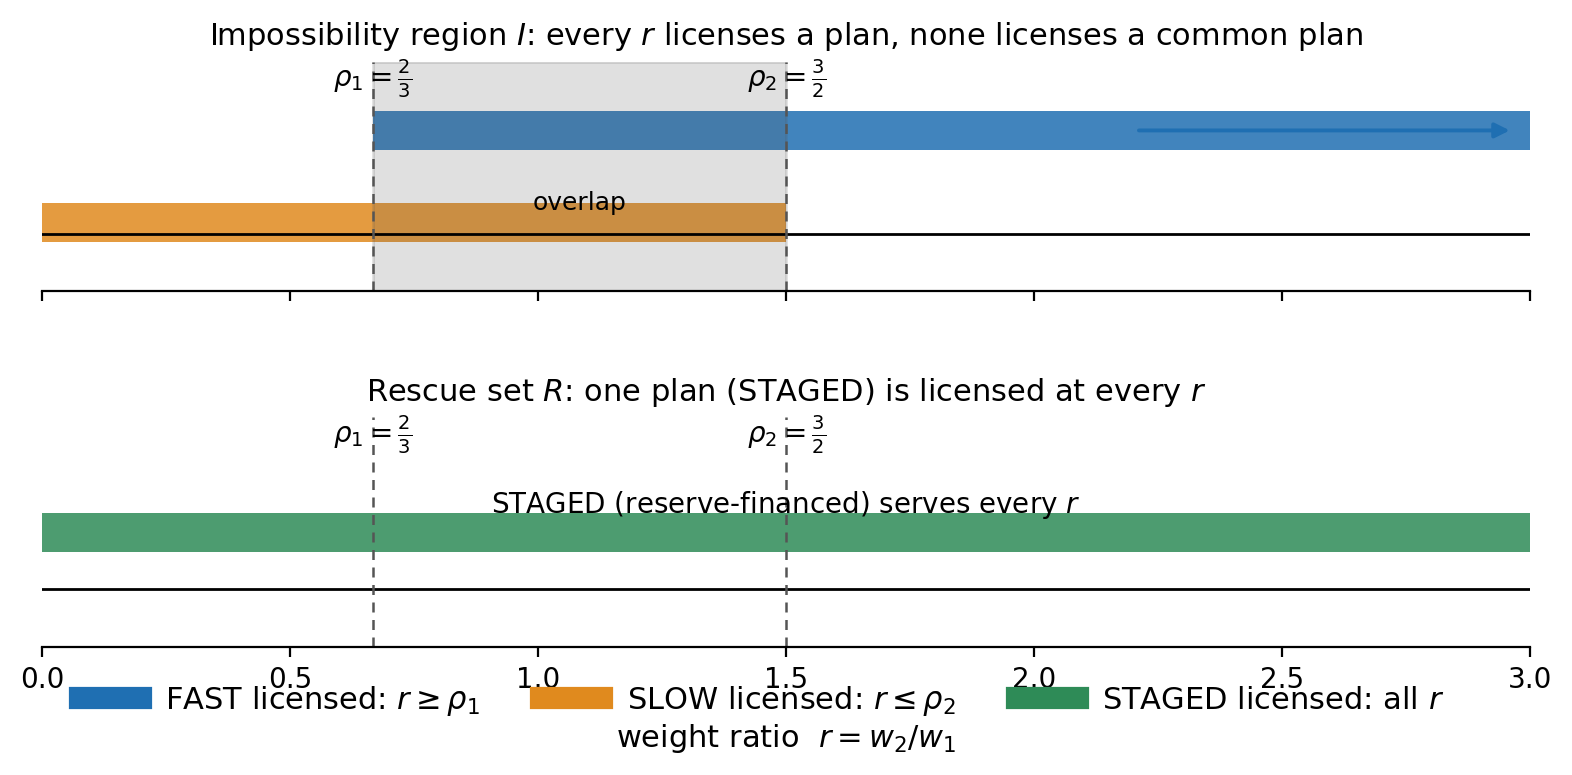
\includegraphics[width=0.9\linewidth]{figS_weight_intervals.png}
\caption{Weight-interval view at the witness point $(x,s_1,s_2)=(\tfrac12,\tfrac65,\tfrac65)$. \act{fast} is licensed exactly for $r\ge\rho_1=\tfrac23$ and \act{slow} exactly for $r\le\rho_2=\tfrac32$. The two intervals together cover every weight ratio $r\ge0$, but neither covers it alone. On the rescue set, \act{staged} supplies the full interval and closes the gap.}
\end{figure}

\section{Verification record}\label{si:verification}

\subsection{The grid verifier}

The companion artifact implements the witness datum in exact integer arithmetic at scale 40 -- no floating point, no tolerances, no randomness. It (i) computes the four plans' worst-case tubes and successors for every state on a $31^3=29{,}791$-state grid; (ii) evaluates the typed, weighted and physical admissibility predicates; (iii) checks the region identities $\Vtyp,\Vweak,\Vphys,R,I,\FP$ of main-text Theorem~2; (iv) checks the threshold identities for $\rho_1,\rho_2$ at the analytically identified critical ratios and their midpoints; and (v) checks the propagation identities of main-text Proposition~3(i) on a hold-prefixed horizon. All 25 checks pass; re-execution reproduces outputs exactly. The certification level is exact finite rational verification -- rigorous for the finite rational computation and distinct from the analytic proofs of the continuum theorems.

\begin{table}[!htbp]
\centering\small
\caption{Claim layers and what establishes each.}
\begin{tabularx}{\textwidth}{@{}>{\raggedright\arraybackslash}p{0.24\textwidth}XX@{}}
\toprule
Claim layer & What is established & By what \\
\midrule
Continuum statements & exact identities and inequalities on the datum & main-text Appendices A--B; SI S2 \\
Finite rational instances & classifications on enumerated grids & deterministic exact computation (six check lists) \\
Theorem layer & the core results at an ordered-field interface & Lean 4 module (199 theorems) \\
Empirical claims & none & -- \\
\bottomrule
\end{tabularx}
\end{table}

\subsection{The 25-check enumeration}

Each entry quotes the check's recorded name from the committed results file (\texttt{research\_program/} \texttt{paper1\_instantiation/} \texttt{typed\_false\_positive\_instantiation.json}; execution of 2026-08-28; deterministic; exit 0) and the main-text claim it maps to. The artifact's tokens ``FP'' and ``FP0'' name the discrepancy region $\Q$.
\begin{enumerate}[leftmargin=2em,itemsep=1pt]
\item \emph{FAST breakpoint table exact (dip at t=1/2, recovery at t=1)} -- the \act{fast} row of main-text Table~5.
\item \emph{STAGED breakpoint table exact (linear spend/growth)} -- the \act{staged} row.
\item \emph{per-coordinate exact ranges = breakpoint extremes (piecewise monotone)} -- every worst-case tube is the exact visited set.
\item \emph{worst-case dip constants: benign 3/2, adverse 2, floor threshold 2} -- the disturbance convention.
\item \emph{machine typed-feasibility == \{x>=1\} $\cup$ \{s1>=2\} $\cup$ \{s2>=2\} on every grid state} -- Theorem~2(1).
\item \emph{machine all-weights admissibility == \{x>=1\} $\cup$ \{s1+s2>=2\} on every grid state} -- Theorem~2(2).
\item \emph{FAST/SLOW per-weight safety biconditionals confirmed on every grid state (dense r-grid)} -- Theorem~2(6).
\item \emph{boundary weights exact: FAST safe at r=rho\_1, SLOW safe at r=rho\_2 (witness state (1/2, 6/5, 6/5))} -- Theorem~2(6).
\item \emph{machine endpoint-only feasibility == all of X\_0 on every grid state} -- Theorem~2(3).
\item \emph{typed $\Rightarrow$ all-weights-aggregate $\Rightarrow$ endpoint-only (no violations on the grid)} -- Proposition~1(i).
\item \emph{false-positive set nonempty on the grid} -- Theorem~2(4); 1,900 grid states in the set.
\item \emph{interior witness (1/2, 6/5, 6/5): aggregate-feasible for every critical weight, typed-INfeasible, endpoint-feasible} -- Theorem~2(4)--(5).
\item \emph{witness is an interior point (all $\pm$0.1 neighbors remain in FP)} -- Theorem~2(4).
\item \emph{endpoint-only witness (1/2, 1/10, 1/10): endpoint-feasible, aggregate-INfeasible (no action safe at w=(1,1))} -- Theorem~2(5).
\item \emph{aggregate-vs-typed strictness witness (the FP interior point above)} -- Theorem~2(5).
\item \emph{r=1/2: SLOW-only (FAST unsafe, SLOW safe)} -- Theorem~2(6).
\item \emph{r=1: both plans safe} -- Theorem~2(6).
\item \emph{r=2: FAST-only (SLOW unsafe, FAST safe)} -- Theorem~2(6).
\item \emph{E\_typ = $\cap$\_w E\_w = $\varnothing$ machine-verified (no action serves every critical weight)} -- Proposition~1(ii) on the witness.
\item \emph{R witness (3/2, 6/5, 6/5): typed-transformable via STAGED (bridging plan at physical cost c=1)} -- Theorem~2(7).
\item \emph{I witness (1/2, 6/5, 6/5): all four actions rejected, each with its exhibited violated constraint (negative-certificate form)} -- Theorem~2(7).
\item \emph{rescue split verified on the whole grid: FP0$\cap$\{x>=1\} typed-feasible via STAGED; FP0$\cap$\{x<1\} typed-infeasible} -- Theorem~2(4), (7); Proposition~5.
\item \emph{stage-0 hierarchy holds and regions are preserved through two hold intervals (every grid state)} -- Proposition~3(i).
\item \emph{FP strictness witness survives the holds at stage 0} -- Proposition~3(i).
\item \emph{endpoint-only strictness witness survives the holds at stage 0} -- Proposition~3(i).
\end{enumerate}

\subsection{The other check lists and the Lean module}

The six check lists are not pooled (the programme's non-pooling policy): grid verifier 25; benchmark script 24 (every quoted value of S5); $\sigma$-ladder verifier 57; off-diagonal closure 50; continuum slice closure 44; common-shock verifier 77 (with the 676-state handshake under the action-indexed class and $5{,}000$-state grids under the common class). Each is a fail-loud exact-arithmetic script with a committed byte-reproducible run log.

The Lean~4 module \texttt{Formalizations/P1\_AssessmentSeparation.lean} (programme repository, directory \texttt{lean/}; 199 theorems; \texttt{lake build} green; zero \texttt{sorry}; zero added axioms) formalises: the witness datum exactly (worst-case tubes as predicates on visited states, endpoint sets, destination-labelled successors); main-text Theorem~2(1)--(7) in full (the three accepted-set identities, $\FP=I$ with its interior witness, both strictness witnesses, the thresholds with the overlap law $\rho_2\ge\rho_1\iff s_1+s_2\ge2$, the rescue split with all four exhibited violations); Lemma~2 and Proposition~1 (the fourfold chain and the full-cone identity) on the datum; Theorem~3(i),(iii) and Proposition~4; the handshake identity and the collapse convention with its rational witness; the master-equation reductions for $\theta>0$, $\theta<0$ (averaging argument at an abstract power interface) and $\theta=0$ (the swap-product identity $F\cdot S=s^2-1$, master row $s^2\ge2$); and Theorem~4(ii)--(iii): the $\theta=1$ rung accepts every gap state, the Leontief identification $\mathcal V^0=\Vtyp$, the false-certification witnesses (the harmonic member's Fibonacci pair and the whole interval $[13/8,2)$; the $\sigma=1/4$ rung at $9/5$; the $\forall m$ family, every $\sigma=1/(m+1)$ false-certifying $[2-2^{-(m+1)},2)$ via a Bernoulli bound; the $\sigma=2$ rung's exact floor $5/4$ as an iff; the $\sigma=3$ rung at the witness point with the bracket $\sigma^*\in(2,3]$; the $\sigma=1$ witness $3/2$ and the $\sqrt2$ floor's bracket $141/100$), and the two-sided summary that only Leontief is uniformly safe. The theorems are proved at an ordered-field interface of which the real-number statements are the instance; the module's comments use the previous edition's result numbers (map in S1).

\section{Positioning notes, per literature}\label{si:positioning}

\paragraph{Commensurability} The foundation statement that values may be only weakly comparable -- and that this incommensurability is constitutive of ecological economics -- is due to Martinez-Alier, Munda and O'Neill (1998). The main article's operators give one formal model of the distinction that paper draws between strong and weak commensurability.

\paragraph{Maximin and indicator formulations} The characterisation of which sustainability criteria admit indicator representations, and the role of maximin and MSY-type reasoning in making strong sustainability operational, are developed in Martinet (2011), Cairns and Martinet (2014) and Doyen and Gajardo (2020). Doyen and Gajardo (2020) show that the multicriteria maximin value is the solution of a static Pareto problem over the viability kernel -- the strongest formal statement in the literature of the position, strong sustainability as constraint viability rather than optimality, that the typed operator formalises.

\paragraph{Compensability in multi-criteria decision analysis} Compensability analysis is established in MCDA, including the explicit mapping of compensatory aggregation to weak sustainability and outranking methods to strong sustainability (Cinelli, Coles and Kirwan, 2014; Sch\"ar, Pohl and Geldermann, 2025). Scalarization-dependent optimal policies are a staple of multi-objective optimisation. Static scalarization limitations -- weighted sums cannot reach nonconvex parts of Pareto fronts (Das and Dennis, 1997) -- act through frontier geometry under a single optimisation, a mechanism distinct from the action-quantifier mechanism.

\paragraph{Acceptance semantics and decision aiding} The protocols of main-text Table~1 are decision-aiding constructs: each specifies the rule by which a composite reading sorts a transition into the accepted or rejected category -- the sorting problematic of decision aiding (Roy, 1996; Vincke, 1992). Under the weight-adaptive rule a transition is accepted when every weighting licenses some plan, possibly a different plan for each weighting; the licensing thresholds are then the verdict's exact weight-sensitivity intervals, the acceptance-side analogue of the sensitivity analyses applied to composite-indicator rankings (Nardo et al., 2008). The preference-elicitation background is multi-attribute value theory's substitution rates (Keeney and Raiffa, 1976) and the incommensurable-criteria treatment of sustainable development (Munda, 2005).

\paragraph{Viability and robust control} The backward recursion is a typed instance of robust-predecessor, reach--avoid, capture-basin and hybrid-reachability constructions (Aubin, 1991; Aubin, Bayen and Saint-Pierre, 2011; Saint-Pierre, 1994; Lygeros, Tomlin and Sastry, 1999; Aubin and Catt\'e, 2002), with fisheries a canonical application (De Lara and Doyen, 2008; Doyen et al., 2012). The blend/time-sharing pair is the pure/mixed structure of the assessor--planner game (von Neumann, 1928; Sion, 1958), whose reach--avoid form is the discriminating kernel of Cardaliaguet (1996), and the here-and-now/wait-and-see distinction of adjustable robust optimisation (Ben-Tal et al., 2004).

\paragraph{Planetary boundaries and the safe-and-just space} The typed operator is a formal idealisation of the separate-boundary reading underlying the Planetary Boundaries framework (Rockstr\"om et al., 2009; Steffen et al., 2015), and the same separately-checked-floor logic underlies the safe-and-just-space literature (Raworth, 2012; O'Neill et al., 2018; Fanning et al., 2022). Boundary processes interact and amplify human impacts (Lade et al., 2020), which is why the coupled disturbance regime of S4 is not a remote possibility. The main theorem provides a formal model of \emph{one reason} a noncompensatory stance may be adopted; it does not prove that planetary boundaries ought to be noncompensatory, which is a normative and scientific-design question.

\section{Framework extensions deposited at partial status}\label{si:framework}

The previous supplementary file of this paper, \texttt{paper1\_supplementary\_v12.md} (deposited with the code), carries a set of framework extensions that the main article does not use in any proof. They are summarised here with their declared status; the full text remains in the deposit.

\paragraph{The named record (status: definition)} A sustainability-assessment model declares a thirteen-field record $\mathfrak S=(T,Z,S_{st},B_{out},V,\Gamma,O,A,C,R,D,K,P)$: type system; state space; stock--flux structure; boundary interface; constitutive laws; service--technology correspondence; observation operator; assessment operator (the subject of the main article); command architecture; deployment/reset architecture; disturbance class; safe-and-just set; policy class. Four uncertainty levels (parameter, observation/assessment, process disturbance, structural) and four model maps (specialisation, exact projection, approximation, singular reduction) complete the layer; claims transfer only along declared maps. The witness datum instantiates the record field by field (three typed coordinates, the phase space $(q,x,s_1,s_2)$, the linear spend/growth flows, the four plans, exact observation, the typed operators, single-command architecture, the destination reset $s\mapsto s+e$, the two-element disturbance class, $K=S_0$, the four-element menu). Every statement carries a status (definition, identity, theorem, conditional theorem, conjecture, counterexample) under two rules: no promotion, no silent transfer. Ten typed failure classes (material inconsistency; physical, epistemic, authority, implementation and temporal infeasibility; recovery, architecture-transition and model-credibility failure; normative incompatibility) discipline verdicts to name the earliest discharged obstruction.

\paragraph{Governance constructors (status: framework extension, partial)} Governance instruments enter as constructors with declared support -- the record fields they may alter -- so that composition is auditable and noncommutation can be proved; the primitive constructors are caps, floors, taxes, exclusions, leaks, observation reforms and restrictions. Restriction of the action correspondence obeys one-sided monotonicity of existential viability kernels, layered along an implementability ladder $U_{\mathrm{impl}}\subseteq U_{\mathrm{inst}}\subseteq U_{\mathrm{tech}}\subseteq U_{\mathrm{theor}}$; a viability result over a theoretical class does not transfer downward. A commons-obstruction theorem (scalar stock $\dot S=g(S)-H$; a uniform negative drift margin $\varepsilon>0$ on a strip above $S_{\min}$ under the implemented Nash feedback; every trajectory entering the strip reaches $S_{\min}$ within $a/\varepsilon$, and exits below it if the drift persists at the boundary) is summarised from the companion obstruction calculus with its conditions explicit.

\paragraph{Intergenerational extension (status: framework extension)} A generation structure assigns closed per-generation constraint sets $V^{(k)}$. Stationary equivalence with ordinary viability holds only under stated restrictions (no inheritance, resets or generation-specific policy classes). Nested impossibility: if trajectories are forward complete and confined to a compact set, each $V^{(k)}$ is closed, and the sets are nested decreasing with empty intersection, then no intergenerationally viable path exists (an $\omega$-limit argument); the theorem does not establish that every finite horizon is satisfiable, which requires a separate example.

\paragraph{Composition extension (status: conditional / incomplete)} An effort-scale invariance in a registered delay-dynamics family, a yield-gap soft-minimum estimate and a ``coupling creates viability'' example are recorded as conditional or not reproducible as written, each with the missing ingredients listed; the two-sided lesson -- composition can create or destroy viability -- is retained as the architectural point.

\paragraph{Application note: planetary boundaries (status: interpretive)} The typed operator supplies a formal model of the separate-boundary reading only; see S8.

\paragraph{Declared conjectures (status: conjecture; none executed)} Nine conjectures with falsification designs: compositional sustainability; transformability (a resource-cost characterisation analogous to $\kappa^*$); capacity-leading failure; bottleneck--robustness; boundary-expansion reversal; distributional dynamics (the gap is largest when floors are negatively correlated across the disturbance class); correlated-disturbance amplification; maintenance suppression; efficiency--scale interaction. Each is governed by preregistration restrictions; no conjecture is rescued by post-hoc state augmentation.

\section*{References cited in the Supplementary Information}
\begin{itemize}[leftmargin=1.5em,itemsep=1pt]
\item Abaee, A. (2026a). An obstruction calculus for viability under incomplete observation. Zenodo. \url{https://doi.org/10.5281/zenodo.22552616}.
\item Abaee, A. (2026c). Does a surplus-production ladder improve forecasts of Northern cod? A scored test on NAFO 2J3KL. Zenodo. \url{https://doi.org/10.5281/zenodo.22553609}.
\item Abaee, A. (2026d). Verification code and figure pipeline for ``Aggregate indices and transition safety''. figshare. \url{https://doi.org/10.6084/m9.figshare.33764023}.
\item Abaee, A. (2026e). Delay-induced regime change in harvested stocks: the mobilising and protective channels of institutional feedback, and the review interval as control. Zenodo. \url{https://doi.org/10.5281/zenodo.22554217}.
\item Aubin, J.-P. (1991). \emph{Viability Theory}. Birkh\"auser, Boston. Aubin, J.-P., Bayen, A.~M., and Saint-Pierre, P. (2011). \emph{Viability Theory: New Directions}, 2nd ed. Birkh\"auser. Aubin, J.-P., and Catt\'e, F. (2002). \emph{Set-Valued Analysis}, 10(4), 379--416.
\item Ben-Tal, A., Goryashko, A., Guslitzer, E., and Nemirovski, A. (2004). \emph{Mathematical Programming}, 99(2), 351--376.
\item Cairns, R.~D., and Martinet, V. (2014). \emph{European Economic Review}, 69, 4--17.
\item Cardaliaguet, P. (1996). \emph{SIAM Journal on Control and Optimization}, 34(4), 1441--1460.
\item Cinelli, M., Coles, S.~R., and Kirwan, K. (2014). \emph{Ecological Indicators}, 46, 138--148.
\item Das, I., and Dennis, J.~E. (1997). \emph{Structural Optimization}, 14, 63--69.
\item Dearing, J.~A., et al. (2014). Safe and just operating spaces for regional social-ecological systems. \emph{Global Environmental Change}, 28, 227--238.
\item De Lara, M., and Doyen, L. (2008). \emph{Sustainable Management of Natural Resources}. Springer. Doyen, L., et al. (2012). \emph{Ecological Economics}, 75, 32--42. Doyen, L., and Gajardo, P. (2020). \emph{Natural Resource Modeling}, 33(3), e12250.
\item DFO (2016). \emph{Stock Assessment of Northern Cod (NAFO Divs.\ 2J3KL) in 2016}. CSAS Science Advisory Report 2016/026.
\item Fanning, A.~L., O'Neill, D.~W., Hickel, J., and Roux, N. (2022). \emph{Nature Sustainability}, 5(1), 26--36.
\item Keeney, R.~L., and Raiffa, H. (1976). \emph{Decisions with Multiple Objectives}. Wiley.
\item Lade, S.~J., et al. (2020). \emph{Nature Sustainability}, 3(2), 119--128.
\item Lygeros, J., Tomlin, C., and Sastry, S. (1999). \emph{Automatica}, 35(3), 349--370.
\item Martinet, V. (2011). \emph{Journal of Environmental Economics and Management}, 61(2), 183--197.
\item Martinez-Alier, J., Munda, G., and O'Neill, J. (1998). \emph{Ecological Economics}, 26(3), 277--286.
\item Munda, G. (2005). In \emph{Multiple Criteria Decision Analysis: State of the Art Surveys}. Springer, 953--986.
\item Nardo, M., et al. (2008). \emph{Handbook on Constructing Composite Indicators}. OECD.
\item O'Neill, D.~W., Fanning, A.~L., Lamb, W.~F., and Steinberger, J.~K. (2018). \emph{Nature Sustainability}, 1(2), 88--95.
\item Raworth, K. (2012). \emph{Oxfam Policy and Practice: Climate Change and Resilience}, 8(1), 1--26.
\item Rockstr\"om, J., et al. (2009). \emph{Nature}, 461, 472--475. Steffen, W., et al. (2015). Planetary boundaries: Guiding human development on a changing planet. \emph{Science}, 347(6223), 1259855.
\item Roy, B. (1996). \emph{Multicriteria Methodology for Decision Aiding}. Kluwer. Vincke, P. (1992). \emph{Multicriteria Decision-Aid}. Wiley.
\item Saint-Pierre, P. (1994). \emph{Applied Mathematics and Optimization}, 29, 187--209.
\item Schaefer, M.~B. (1954). \emph{Inter-American Tropical Tuna Commission Bulletin}, 1(2), 23--56.
\item Sch\"ar, S., Pohl, E., and Geldermann, J. (2025). \emph{Journal of Multi-Criteria Decision Analysis}, 32, e70013.
\item Sion, M. (1958). \emph{Pacific Journal of Mathematics}, 8(1), 171--176. von Neumann, J. (1928). \emph{Mathematische Annalen}, 100, 295--320.
\end{itemize}

\end{document}
